\chapter{Proposta}\label{cap2}
\section{Usuários}
A plataforma Moodle possuem por padrão três tipos de perfil de usuário: (i) Administrador; (ii) Professor; e (iii) Aluno.  A plataforma pode ser aplicada em diversos contextos, tais como Universidades, Escolas de Ensino Médio, Escolas Primárias, Organizações Militares, Companhias privadas, entre outros. No entanto, este trabalho tem como usuários iniciais  professores e estudantes universitários do s cursos de Engenharia de Software, Engenharia de Energia, Engenharia Eletrônica, Engenharia Automotiva e Engenharia Aeroespacial. Lotados no Campus Gama da Universidade de Brasília (UnB). Posteriormente, Alunos e professores dos demais Campus – Ceilândia, Planaltina e Darcy Ribeiro.

\section{Terminologias Existentes}

\subsection{Tesauros}
O tesauro a seguir é referênte à funcionalidades do moodle. Foi desenvolvipelo por Norazah Yusof e Andi Besse Firdausiah Mansur em inglês, um vez que o processo de tradução pode trazer dano ao significado do tesauro, será exposto e utilizado na forma nativa do desenvolvimento.

\begin{otherlanguage*}{english}

\begin{description}
  \item[Assignment] \hfill Reflect the task that given to student for each course to measure student performances.
  \item[Blog] \hfill Moodle activity that can be used for expressiveness and conversation with other people.
  \item[Chat] \hfill Moodle activity that can facilitate people to meet in certain virtual room and communicate each other directly through message.
  \item[Choice] \hfill Poll system
  \item[Database] \hfill Sharing data
  \item[Feedback] \hfill The comment or criticism from user
  \item[Forum] \hfill Moodle activity that provide discussion and considered as one of great communication media
  \item[Quiz] \hfill Moodle activity that handled variety of Quiz such as multiple choice or true/false
  \item[Wiki] \hfill Moodle activity that provide user to work together as collaborative team

\end{description}
\end{otherlanguage*} 

\subsection{Ontologias Existente}
A ontologia na qual esse projeto se baseia, foi desenvolvida pela Universidade da Malaysia. Essa ontologia, estrutura, ontologicamente, a plataforma moodle. Os pontos levantados pela ontologia são as relações entre integrantes da rede acadêmica - professores, alunos, coordenadores - e as atividades desenvolvidas por cada integrate.

As relações estabelecidas, pela ontologia, foram relações diretas e indiretas entre professores-estudante, estutante-estudante, professor-atividade e estutande-atividade, classificadas em quatro tipo de propriedade: funcional, inversa, simetrica e transitiva. 

\subsection{Propriedade Funcional}
A propriedade funcional é limitada à um relacionamento de um indivíduo para outro indivíduo determinado como ilustrado na Figura 1. Neste caso, as propriedades de tipo de dados funcional estudante: Hasgroup é considerado como propriedades funcionais. 


 \begin{figure}[ht]
  \centering
    \includegraphics[keepaspectratio=true,scale=0.5]{figuras/sim.eps}
  \caption{Exemplo de propriedade funcional - Hasgroup}
\end{figure}


\subsection{Propriedade Inversiva}
As propriedades que descrevem o indivíduo são como o inverso do outro indivíduo. Neste estudo, HasStudent é propriedade inversa de HasTeacher, como mostrado na Figura 2.

 \begin{figure}[ht]
  \centering
    \includegraphics[keepaspectratio=true,scale=0.5]{figuras/fun.eps}
  \caption{Exemplo de propriedade inversa - HasTeacher and HasStudent}
\end{figure}

Assim é possivel determina os relacionamentos em ambas as direções de pesquisa, ou seja, temos a capacidade de pesquisar tanto quais estutant estudaram com um professor especifio e também quais professores deram aula para um determinado estudante.

\subsection{Propriedade Simétrica}
A propriedad de simetria é a propriedade que define semelhanças em comum com dois elementos, como mostrado na figura 3. Um exemplo de propriedade simétrica é a Hasclassmate.


 \begin{figure}[ht]
  \centering
    \includegraphics[keepaspectratio=true,scale=0.5]{figuras/inv.eps}
  \caption{Exemplo de propriedade simétrica - Hasclassmate}
\end{figure}

Dessa forma é possivel determinar grupos de integrantes com o mesmo perfil.

\subsection{Propriedade Trasitiva}
Relação transitiva é a que se estabelece entre três integrantes de tal forma que se o primeiro tem relação com o segundo e este tem relação com um terceiro, então o primeiro elemento tem relação com o terceiro. A figura 4 exemplifica essa relação na ontoliga do moodle


 \begin{figure}[ht]
  \centering
    \includegraphics[keepaspectratio=true,scale=0.5]{figuras/tra.eps}
  \caption{Exemplo de propriedade trasitiva- HasGroupmate}
\end{figure}

\section{Descrição do Ambiente Web: Plataforma Moodle}

O desenvolvimento da plataforma Moodle foi liderado pelo Australiano Martin  Dougiamas e seu primeiro protótipo foi publicado em novembro de 2001. Sua versão 1.0 foi lançada em agosto de 2002. O fato de a plataforma ser um Software Livre contribuiu no seu crescimento e expansão, visto que esta ganhou atenção de diversos programadores que criaram novos temas e traduziram-na para diversos idiomas.   A concepção e desenvolvimento da plataforma Moodle é guiada por uma  “pedagogia social construcionista” \cite{moodle}.
Onde esta, apoiada por quatro grandes conceitos  : (i) Construtivismo, relacionado à construção do conhecimento através da interação entre as pessoas; (i) Construcionismo - Relacionado à eficácia do aprendizado quando um conhecimento construído pode ser experimentado por outras pessoas; (iii) Construtivismo Social - É o sentido mais amplo do item anterior, este está relacionado à criação de culturas colaborativa de conhecimentos; (iv) Conectado e Separado - De acordo com a documentação da plataforma, este conceito está relacionada as motivações das pessoas dentro de uma discussão. Onde estas podem ter três tipos de comportamentos. (a) Comportamento separado, quando há tentativa de permanecer objetiva e defender suas próprias ideias usando lógica para encontrar falhas nas idéias dos outros envolvido nas discussões; (b) Comportamento conectado, quando a pessoa tem um comportamento mais ouvinte e tem mais aceitação à subjetividade, ela tende a ouvir a fazer perguntas apresentando um esforço para compreender o outro ponto de vista; (c) Comportamento construído, quando uma pessoa apresenta mais sensibilidade a ambas abordagens e possui capacidade de escolher qualquer um deles. Segundo a documentação \cite{moodle}, uma quantidade saudável de comportamento conectado dentro de uma comunidade de aprendizagem é um estimulante poderoso, pois além de aproximar as pessoas pode promover reflexões mais profundas e re-exame das crenças existentes.



\section{Cronograma}
A criação das atividades desse cronogrma foram baseadas no plano de ensino da disciplina Tópicos especiais em Eng. de Software. 

 \begin{figure}[ht]
  \centering
    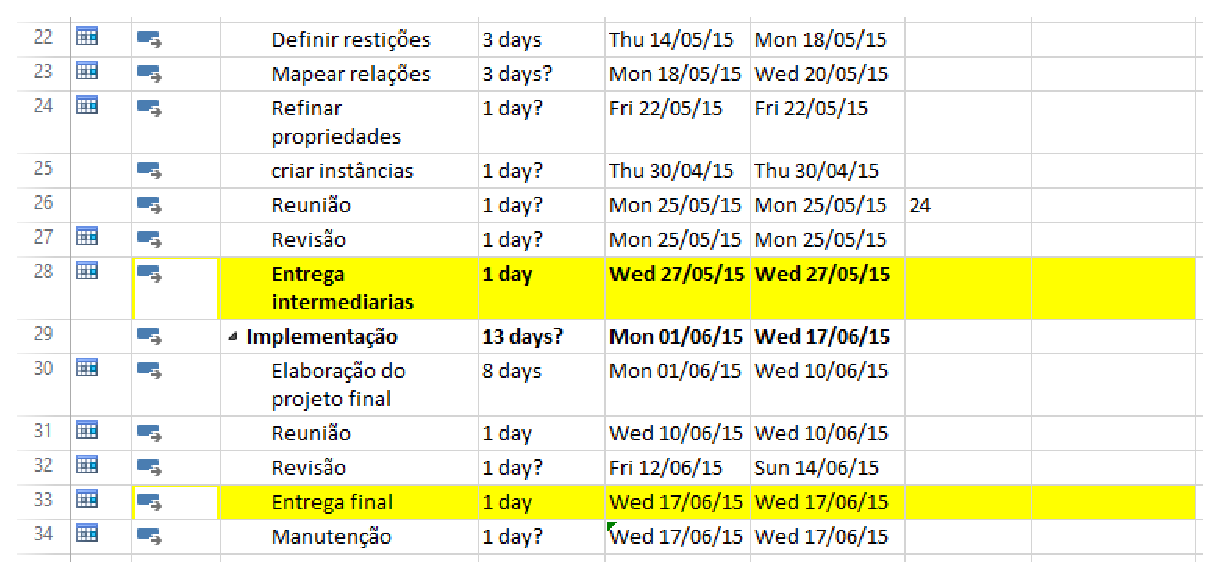
\includegraphics[keepaspectratio=true,scale=0.5]{figuras/cronograma.eps}
  \caption{Cronograma do projeto}
\end{figure}


\chapter{Conceitos Abordados na Disciplina}\label{cap3}

\section{Web Sintática vs. Web Semântica}

No inicio da internet, os web sites criados eram voltado à apresentação de conteúdo, cuja sua interpretação ficava delegada aos seres humanos. As páginas web pouco continha informações sobre si mesma. Estas páginas em grande quantidade trazem um grande problema para mecanismos de busca tais como : (i) baixa precisão da busca, mesmo quando a quantidade de páginas retornadas é grande; (ii) resultados sensíveis ao vocabulário, em alguns casos até a ordem em que as palavras são digitadas influenciam o resultado da busca; e (iii) resultados são páginas individuais, onde muitas páginas de resultado são do mesmo site.  Karin Breitman afirma em seu livro “Web Semântica - A internet do futuro”, que todos esses problemas apresentados são oriundos da Web Sintática. E com o crescimento exponencial da web, viu-se a necessidade em otimizar a organização da informação para que o computador seja capaz de compreender o conteúdo de uma web site e ao fazermos uma busca, este computador selecione as páginas que possuem o conteúdo mais preciso. E assim, finalmente, responder a questão : Porque os computadores não podem realizar esse trabalho para nós?.

Pesquisadores da Inteligência artificial vêm propondo uma série de modelos de organização da internet. O objetivo central é organizar a informação de maneira padronizada, como é feito na classificação dos seres vivos pelo biólogos, dessa maneira contribuir na facilitação em localizar uma informação. A organização dos conteúdos presente na web possibilita a compreensão deste por computadores, e isso caracteriza a Web semântica. Karin Breitman apresenta em seu livro, temas importantes relacionados à Web Semântica. Tais como: (i) Metadados, que são dados sobre dados e são úteis na indexação de páginas e sites na Web semântica, assim permitindo que outros computadores saibam de que assuntos eles tratam; (ii) Ontologias, são especificações formais e explicitas de conceitualizações compartilhadas. Ontologias são modelos conceituais que servem como base para garantir uma comunicação livre de ambiguidades; (iii) Linguagens da Web semântica, são linguagens que facilitem a publicação de ontologias em um formato que capacitem os computadores a processar sua informação; (iv) Construção de modelos semânticos, consiste em construir ontologias gerais para organização da web; (v) Web Services, são servidores que disponibilizam determinados serviços a serem consumidos por computadores, onde a comunicação pode ser feita através de trocas de arquivos xml ou Json; (vi) Agentes, são softwares autônomos e assíncronos que agem em beneficio de seus usuários, realizando tarefas de buscas e seleção de conteúdos na web, por exemplo, que sejam de interesse de seus usuários; e (vii) Ferramentas, quais ferramentas existentes para se implementar a web semântica.

Karin Breitman diz que a web semântica não é inteligência artificial, pois o conceito de documentos compreensíveis por computadores não implica uma inteligência artificial. Uma vez que a web semântica auxilia a organização do conteúdo, enquanto que uma das vertentes da  inteligência é compreender a linguagem humana. A web semântica não é uma web separada, mas sim uma extensão da web atual.

\section{Metadados}

Metadados são dados sobre dados. São informações sobre um documento: data, autor, editora, etc. A international Federation of Library Associations (IFLA) define metadados da seguinte forma : 
\begin{citacao}
 Metadados são dados sobre dados. O termo se refere a qualquer informação utilizada para identificação, descrição e localização de recursos.
\end{citacao}

A W3C (World Web Consortium) tem uma visão mais voltada para a web semântica. metadados são definidos como “informações para a web que pode ser compreendidas por máquinas”. Segundo Karin Breitman,  o tema metadado ainda está aberto a discussões nas várias comunidades onde ele é utilizado. Uma das consequências mais interessantes da adoção de metadados no contexto da web semântica é a de que a disciplina de Catalogação praticada apenas por curadores de museus ou bibliotecários, passou atualmente para o primeiro plano da pesquisa em ciência da informação. 

\section{Dublin Core}
O Dublin Core é um padrão bastante simples, como pode ser observado a partir do grupo básico de elementos que o compõem. Ele rapidamente se tornou padrão para metadados, e atualmente é um padrão ANSI (ANSI/NISO Z39.85) e norma ISO (ISO Standart 15836-2003 Fevereiro de 2003). Os elementos que compõem o padrão Dublin Core são: 

\begin{itemize}
\item Assunto
\item Título
\item Criador
\item Descrição
\item Editor
\item Outro agente (contribuidor, coautores)
\item Data
\item Tipo de origem
\item Formato
\item Identificador
\item Relacionamento (relação com outro objetos)
\item Fonte
\item Linguagem
\item Cobertura
\item Direitos
\end{itemize}

\section{Framework de Warwick}

Esse padrão surgiu da necessidade de ampliar o Dublin Core, considerado muito simples, pois só disponibiliza um formato para descrição de recursos. Foi então criada uma nova arquitetura, baseada no conceito de um contêiner, que agrega vários tipos de metadados em pacotes separados, onde, nesta arquitetura o Dublin Core é apenas um dos pacotes. Os conceitos básicos de Dublin Core não foram modificados pelo Framework de Warwick, foram apenas adicionados novos elementos: 

\begin{itemize}
\item Descrições específicas do domínio do documento (objeto)
\item Termo e condições de uso do documento
\item Rótulo e gradação do documento
\item Informações de segurança, autenticidade, assinaturas
\item Origem do fornecedor
\item Conjunto de containers para documentos compostos e ponteiros para todas as manifestações, instâncias ou versões do documento
\item Responsável por armazenar o documento
\item Conjunto de descritores do Dublin Core do documento
\end{itemize}

O Framework de Warwick deixa em aberto algumas questões. A primeira é a independência de sintaxe. Cada um dos pacotes (Dublin Core, MARC e Referência Indireta) pode utilizar uma sintaxe diferente, o que não garante que dois pacotes poderão trocar dados entre si. Outro problema é sobre a semântica utilizada. De modo a tratar essas dificuldades, um novo padrão surgiu, o RDF — Resource Description Framework.

\section{Resource Description Framework - RDF}

O RDF é uma linguagem declarativa que fornece uma maneira padronizada de utilizar o XML para representar metadados no formato de sentenças sobre propriedades e relacionamentos entre itens na web. Pode-se intender o RDF como uma implementação do Framework  de Warwick, e uma grande influência do RDF veio da comunidade de Representação do Conhecimento (KR - Knowledge Representation). Estes pesquisadores estão estudando maneiras de representar conhecimento sob um formato que permita às máquinas processá-lo. O RDF foi projetado de modo a representar metadados de recursos web de maneira legisle e processável por máquinas.  Um dos objetivos do RDF é tornar a semântica de recursos web acessível a computadores. Ele vai acrescentar metainformações a esses recursos, de modo a possibilitar às máquinas lidarem com eles de modo inteligente. Em RDF escrevemos frases do tipo Recurso + Propriedade + Valor. Essas partes pode ser compreendidas como o sujeito, o predicado e o objeto de uma sentença.

\section{Ontologias e Ciências da Computação}

A palavra ontologia vem do grego ontos (ser) + logos (palavra). Ontologia, na Filosofia, é a ciência do que é, dos tipos de estruturas dos objetos, propriedades, eventos, processos e relacionamentos em todas as áreas da realidade. Segundo Karin Breitman, a definição de ontologia encontrada mais frequentemente na literatura da web semântica é a proposta pro Gruber: “Ontologia é uma especificação formal e explícita de uma conceitualização compartilhada.” . Contextualização representa um modelo abstrato de algum fenômeno que identifica os conceitos relevantes para o mesmo. Explicita significa que os elementos e suas restrições estão claramente definidos. Formal significa que a ontologia deve ser passível de processamento automático, e compartilhada reflete a noção de que uma ontologia captura conhecimento consensual, aceito por um grupo de pessoas. De maneira mais sucinta, a W3C coloca que ontologias devem promover descrições para os seguintes tipos de conceitos: (i) Classes (ou “coisas”) nos vários domínios de interesse; (ii) Relacionamentos entre essas “coisas”; e (iii) Propriedades ( ou atributos) que essas “coisas” devem possuir. 



 





